\documentclass[11pt, oneside]{article}   	% use "amsart" instead of "article" for AMSLaTeX format
\usepackage{geometry}                		% See geometry.pdf to learn the layout options. There are lots.
\geometry{letterpaper}                   		% ... or a4paper or a5paper or ... 
%\geometry{landscape}                		% Activate for for rotated page geometry
%\usepackage[parfill]{parskip}    		% Activate to begin paragraphs with an empty line rather than an indent
\usepackage{graphicx}				% Use pdf, png, jpg, or eps§ with pdflatex; use eps in DVI mode
								% TeX will automatically convert eps --> pdf in pdflatex		
\usepackage{amssymb}
\usepackage{amsmath}
\usepackage{parskip}
\usepackage{color}
\usepackage{hyperref}

\title{Wicked integrals}
%\author{The Author}
%\section{}
%\subsection*{}
\date{}							% Activate to display a given date or no date

\graphicspath{{/Users/telliott_admin/Dropbox/Tex/png/}}
% \begin{center} 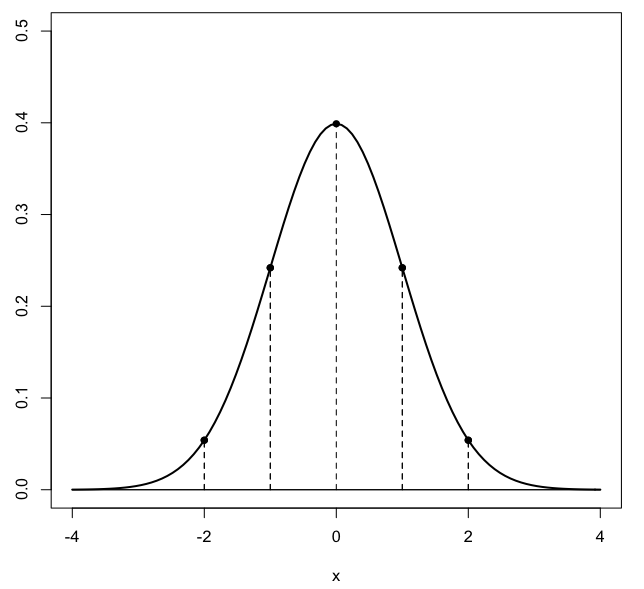
\includegraphics [scale=0.4] {gauss3.png} \end{center}
\begin{document}
\maketitle
\Large
\[ \int_0^{\pi/2} \frac{\sin x}{\sin x + \cos x} \ dx = \ ? \]
Going to the cotangent doesn't help me.

Here's the trick:
\[ \frac{\sin x}{\sin x + \cos x} \]
\[ = \frac{1}{2} \cdot\ \frac{\sin x + \sin x}{\sin x + \cos x} \]
Now, add and subtract $\cos x$ in the numerator!
\[ = \frac{1}{2} \cdot\ \frac{\sin x + \cos x + \sin x - \cos x}{\sin x + \cos x} \]
If you don't see it yet, this should help
\[ = \frac{1}{2} \ [ \ 1 - (\frac{\cos x - \sin x}{\sin x + \cos x}) \ ] \]
But now the term in parentheses, together with $dx$, is
\[ \int \frac{du}{u} \]
So the answer is
\[ I = \frac{1}{2} \ [ \ x - \ln (\sin x + \cos x) \ ] \]
And since $\sin x + \cos x = 1$ at both bounds, the logarithm term is 
\[ \ln 1 = 0 \]
at both bounds, so we get just
\[ = \frac{1}{2} x \ \bigg |_0^{\pi/2} = \frac{\pi}{4} \]

\end{document}  